\documentclass[final]{beamer}
\usetheme{Uchicago}
%\usepackage[orientation=portrait,size=a0,scale=1.4,debug]{beamerposter}
\usepackage[size=custom,width=84,height=111,scale=1.3]{beamerposter}
\usepackage[absolute,overlay]{textpos}
\setlength{\TPHorizModule}{1cm}
\setlength{\TPVertModule}{1cm}

\usepackage{bm} % to get bold greek letters

\title{Genetic architecture of gene expression regulation via orthogonal tissue decomposition}
\author{Heather E. Wheeler\textsuperscript{1,2*}, GTEx Consortium, Nicholas Knoblauch\textsuperscript{3},  Nancy J. Cox\textsuperscript{4}, Dan L. Nicolae\textsuperscript{2}, Hae Kyung Im\textsuperscript{2*}}
%\author{Heather E. Wheeler$^1$, Nicholas Knoblauch$^1$, GTEx Consortium, Dan L. Nicolae$^1$,\\ Nancy J. Cox$^2$, Hae Kyung Im$^{1*}$}
\institute{\small{\textsuperscript{1}Departments of Biology and Computer Science, Loyola University Chicago; \textsuperscript{2}Department of Medicine, University of Chicago, Chicago, IL;\\\textsuperscript{3}Committee on Genetics, Genomics, and Systems Biology, University of Chicago; \textsuperscript{4}Division of Genetic Medicine, Vanderbilt University}}
% \footer{$^\dagger$ Equal contribution \hspace{0.62\textwidth} $^*$ correspondence to \texttt{haky@uchicago.edu}}
\footer{$^*$correspondence to \texttt{hwheeler1@luc.edu} or \texttt{haky@uchicago.edu}}
% \logo{UChicago_REVERSED_WHITE.png}
%\footer{}
\date{}

\newcommand{\VcoordTop}{12}
\newcommand{\VcoordBottom}{55}
\newcommand{\HcoordFirst}{1.5}
\newcommand{\HcoordSecond}{29}
\newcommand{\HcoordThird}{56.5}
\newcommand{\ColWidth}{26}

\bibliographystyle{prwileyj}

\begin{document}
\begin{frame}{} 

%% logo
% 
\begin{textblock}{\ColWidth}(65.5,7.5)%(65.5,7.5)
% \begin{block}{Summary}
	%\includegraphics[width=.66\linewidth]{UChicago_REVERSED_WHITE.png}
	% \end{block}
\end{textblock}


% \begin{textblock}{\ColWidth}(1,11)
% 	\begin{block}{11}
% 	\end{block}
% \end{textblock}

%
% FIRST COLUMN - TOP
%

\begin{textblock}{\ColWidth}(\HcoordFirst,\VcoordTop)

\begin{block}{Summary}
\begin{footnotesize}

For many complex traits, gene regulation is likely to play a crucial mechanistic role given the consistent enrichment of expression quantitative trait loci (eQTLs) among trait-associated variants. In order to fully harness gene regulation mechanisms in future studies of complex traits, we sought to better understand the underlying genetic architecture of the gene regulation traits themselves. We show that local heritability of gene expression (variance in gene expression due to genetic variation within 1Mb of a gene) can be accurately estimated across tissues, but distal heritability cannot be reliably estimated at sample sizes less than 1000. Using both the elastic net and Bayesian sparse linear mixed modeling, we show that for local gene regulation, the genetic architecture is mostly sparse rather than polygenic. Using genome and transcriptome data from the diverse set of tissues available in The GTEx Project, we developed a model called Orthogonal Tissue Decomposition (OTD), which partitions gene expression into cross-tissue and tissue-specific components. Estimates of the local heritability of OTD-generated cross-tissue gene expression have larger magnitude and smaller standard errors compared to single tissue estimates due to the borrowing of information across all samples. We show that genes with high cross-tissue heritability are more likely to have cross-tissue eQTLs, confirming that OTD is capturing the cross-tissue component of gene expression. We also found evidence that genes with large tissue-specific heritability are enriched in common complex disease genes discovered via GWAS. Cross-validated predictors of cross-tissue and tissue-specific expression built here have been added to the PrediXcan (Gamazon, Wheeler, Shah et al. Nature Genetics 2015) database for future investigations of complex traits. In conclusion, local heritability estimates can be reliable obtained across tissues but not the distal component. For local regulation, the architecture is sparse rather than polygenic. Finally, an interesting enrichment of high tissue specific heritability of disease-associated genes merits further investigation.

\end{footnotesize}
\end{block}

\begin{block}{Linear Model for Gene Expression Trait}

\[ Y_g = \sum_{k = \in local}w_{k,g} X_k + \sum_{k = \in distal}w_{k,g} X_k + \epsilon \]

\end{block}

\begin{block}{Prediction Performance vs. Heritability}
	\begin{center}
	\begin{center}
		\includegraphics[width=0.9\textwidth]{plots/Fig3_compareR2_h2_en.png}
	\end{center}
	\end{center}

\bigskip

\end{block}

\begin{block}{Local and Distal Joint Heritability (h$^2$)}
	\begin{center}
		\includegraphics[width=0.5\textwidth]{plots/Fig1.png}
		\includegraphics[width=0.5\textwidth]{plots/Fig2.png}

	\end{center}
 		{\tiny DGN whole blood expression joint (h\textsuperscript{2}). Left: Local (SNPs within 1 Mb of each gene) and distal
 (SNPs that are eQTLs in the Framingham Heart Study on other chromosomes
 {[}FDR \textless{} 0.05{]}) h\textsuperscript{2} for gene expression
 were jointly estimated. (\textbf{A}) Distal h\textsuperscript{2}
 compared to local h\textsuperscript{2} per gene. (\textbf{B}) Local and
 (\textbf{C}) distal gene expression h\textsuperscript{2} estimates
 ordered by increasing h\textsuperscript{2}. The 95\% confidence interval
 (CI) of each h\textsuperscript{2} estimate is in gray and genes with a
 lower bound greater than zero are in blue. Right: Joint h$^2$ estimated with local (SNPs within 1 Mb
 of each gene) and known trans-eQTLs (SNPs that are trans-eQTLs in the
 Framingham Heart Study for each gene {[}FDR \textless{} 0.05{]}).\\}
\end{block}



\end{textblock}

%
% SECOND COLUMN - TOP
%

\begin{textblock}{\ColWidth}(\HcoordSecond,\VcoordTop)

\begin{block}{Orthogonal Tissue Decomposition (OTD)}
	\begin{center}
		\includegraphics[width=\textwidth]{plots/OTD.pdf}
	\end{center}

\end{block}


\begin{block}{Cross-tissue, Tissue-wide and Tissue-specific h$^2$ }
	\begin{center}
		\includegraphics[width=.5\textwidth]{plots/Fig4.png}
		\includegraphics[width=.5\textwidth]{plots/FigS1.png}
		
		\tiny{Left. Cross-tissue compared to tissue-wide h$^2$.
		Right. Cross-tissue compared to tissue-specific h$^2$.}
	\end{center}

\end{block}

\begin{block}{Cross-tissue h$^2$ Estimates Have Lower Error}
	\begin{center}
		\includegraphics[width=0.5\textwidth]{plots/Fig5.png}
		\includegraphics[width=0.5\textwidth]{plots/FigS2.png}
		

	\end{center}
	{\tiny Cross-tissue heritability (h\textsuperscript{2}) compared to
tissue-wide h\textsuperscript{2}. Cross-tissue local
h\textsuperscript{2} is estimated using the cross-tissue component
(random effects) of the mixed effects model for gene expression and SNPs
within 1 Mb of each gene. Tissue-wide local h\textsuperscript{2} is
estimated using the measured gene expression for each respective tissue
and SNPs within 1 Mb of each gene.\\}

\end{block}

\begin{block}{OTD Cross-tissue Expression Correlates with Multi-tissue eQTL Results}
	\begin{center}
		\includegraphics[width=0.9\textwidth]{plots/Fig-CT-entropy.png}
	\end{center}
	{\tiny Entropy of the posterior probabilities from the Flutre et al. (PLOS Genetics 2013) multi-tissue eQTL method compared to the estimates of (left) heritability and (right) PVE of cross-tissue gene expression derived from the orthogonal tissue decomposition. The generalized additive model smoothing line is in red.\\}

\end{block}

\end{textblock}

% T3 THIRD COLUMN - TOP

\begin{textblock}{\ColWidth}(\HcoordThird,\VcoordTop)

\begin{block}{Cross-tissue Expression Has Larger Effective Sample Size}
	\begin{center}
		\includegraphics[width=0.4\textwidth]{plots/OTD-sample-increase.png}
	\end{center}
\end{block}


\begin{block}{OTD Tissue-specific Expression Correlates with Multi-tissue eQTL Results}
	\begin{center}
		\includegraphics[width=0.6\textwidth]{plots/Fig-cor-StephensPr-OTDtsPVE.png}
	\end{center}
	{\tiny Pearson correlation (R) between the posterior probability the top multi-tissue eQTL regulates its gene in a given tissue (eQTL, Flutre et al. method, PLOS Genetics 2013) and the percent variance explained (PVE) of tissue-specific gene expression from the orthogonal tissue decomposition (OTD). Area of each circle is proportional to the absolute value of R.\\}
\end{block}



\begin{block}{Elastic Net Consistent with Sparse Architecture}
	\begin{center}
		\includegraphics[width=0.8\textwidth]{plots/Fig3.png}
	 \end{center}
	 {\tiny Cross-validated predictive performance across the elastic net. (A) 10-fold cross-validated R$^2$ of predicted vs. observed expression in DGN whole blood compared to a range of elastic net mixing parameters ($\alpha$) for genes on chromosome 22 with R$^2 > 0.3$. (B) Predictive R$^2$  difference between LASSO ($\alpha=1$) and several other values of $\alpha$ compared to LASSO predictive R$^2$  for 341 genes on chromosome 22.\\}

\end{block}
\begin{block}{BSLMM Consistent with Sparse Archetecture}
	\begin{center}
%		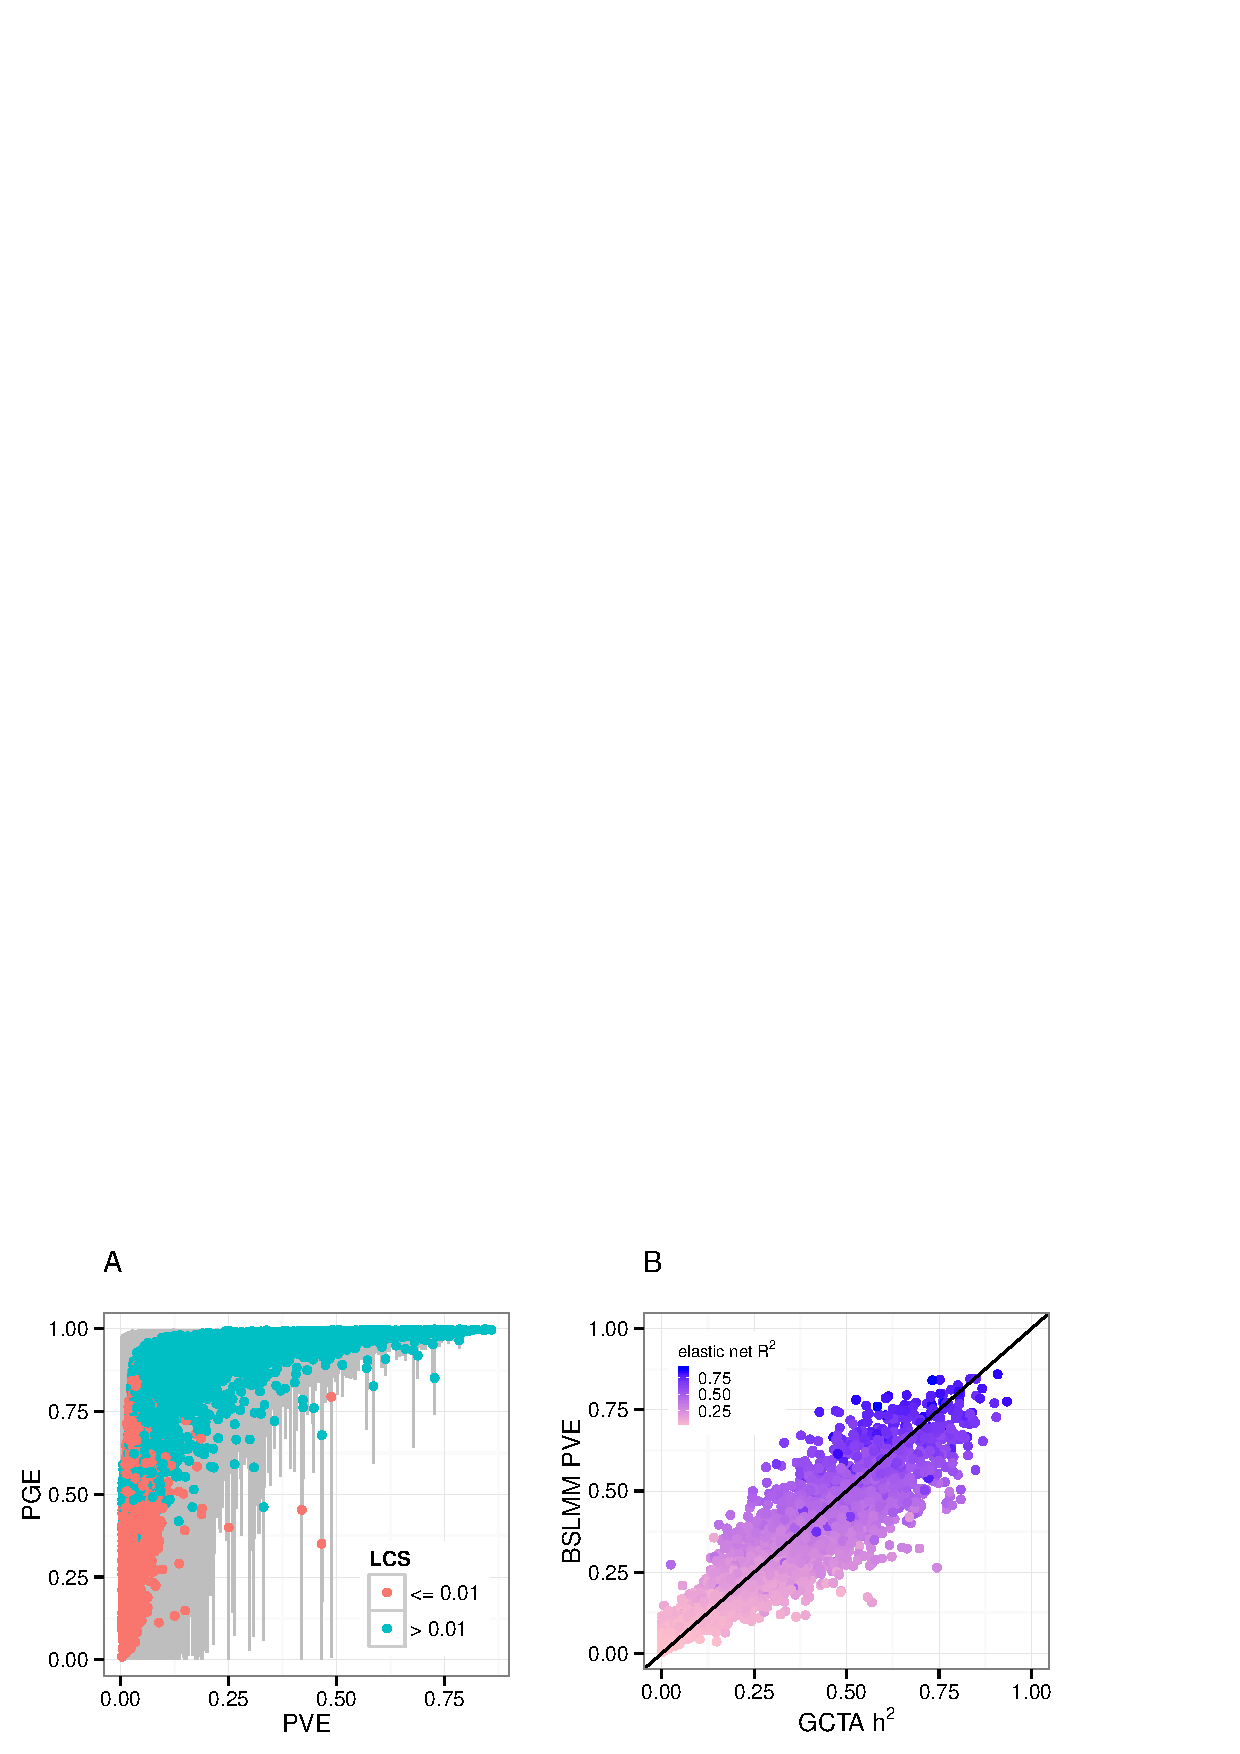
\includegraphics[width=0.5\textwidth]{plots/Fig-DGN-BSLMM.png}
		\includegraphics[width=0.45\textwidth]{plots/Fig-DGN-BSLMM-A.png}
		\includegraphics[width=0.45\textwidth]{plots/Fig-DGN-BSLMM-B.png}\\
		\includegraphics[width=0.45\textwidth]{plots/Fig-DGN-BSLMM-C.png}\\
	 \end{center}
	{\tiny (A) Bayesian Sparse Linear Mixed Model (BSLMM)-estimated PVE (total proportion of variance explained) compared to GCTA-estimated heritability per gene (R=0.96) (B) Comparison of median PGE (proportion of PVE explained by sparse effects) to median PVE (total proportion of variance explained) for expression of each gene. The 95\% credible set of each PGE estimate is in gray and genes with a lower credible set (LCS) greater than 0.01 are in blue. (C) Comparison of the median number of SNPs included in the model of each gene to median PVE. The 95\% credible set of each SNP-number estimate is in gray and genes with a median of 10 or fewer SNPs are in blue.\\}
\end{block}


\begin{block}{Acknowledgements}
\begin{tiny}

NCI/K12CA139160; PAAR (NIH/NIGMS grant UO1GM61393); PGRN Statistical Analysis Resource (U19 HL065962); Genotype-Tissue Expression project (GTeX) (R01 MH101820 and R01 MH090937); University of Chicago DRTC (Diabetes Research and Training Center; P30 DK20595, P60 DK20595); The Conte Center for Computational Neuropsychiatric Genomics (P50MH094267); Integrated GWAS of complex behavioral and gene expression traits in outbred rats (P50DA037844).\\

\bigskip

\textbf{Data Sources}

GTEx (\url{gtexportal.org}), DGN (Depression Genes and Networks, \url{nimhgenetics.org})

\bigskip

\textbf{References}

Gamazon ER*, Wheeler HE*, Shah KP* et al. A gene-based association method for mapping traits using reference transcriptome data. Nature Genetics. 2015; 47: 1091-1098. doi:10.1038/ng.3367 *Contributed equally.

\bigskip

Flutre T et al. A statistical framework for joint eQTL analysis in multiple tissues. PLoS Genetics. 2013; 9: e1003486. doi:10.1371/journal.pgen.1003486

\end{tiny}


\end{block}

\end{textblock}



\end{frame}

\end{document}
